% Source - https://tex.stackexchange.com/a/28286
% Posted by Peter Grill, modified by community. See post 'Timeline' for change history
% Retrieved 2026-11-16, License - CC BY-SA 3.0

\documentclass{standalone}

\usepackage{tikz}
\usetikzlibrary{3d}

\usepackage{xcolor}
\pagecolor{white}

\begin{document}

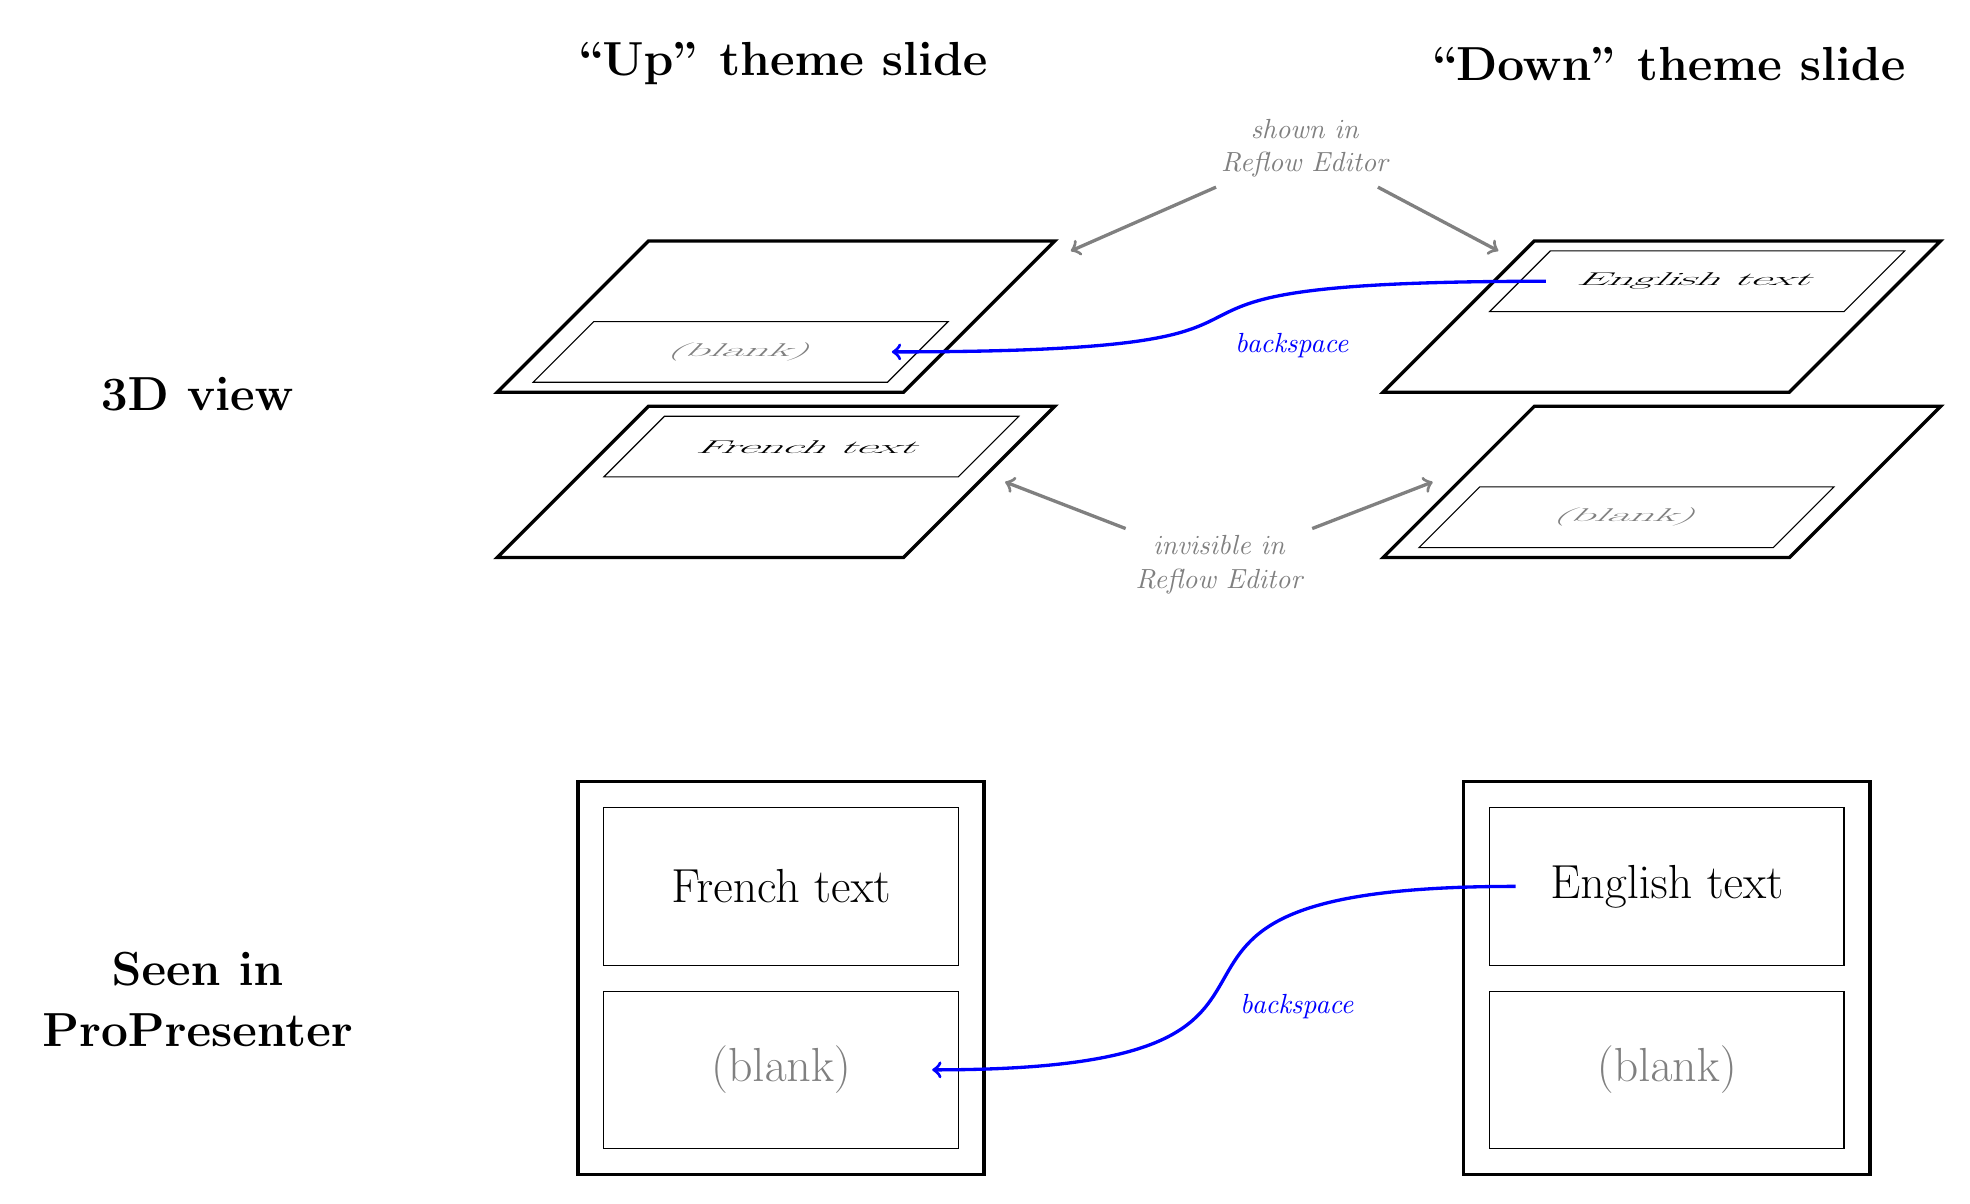
\begin{tikzpicture}

\LARGE

\newcommand{\Width}{4.5}
\newcommand{\Height}{2.1}
\newcommand{\Depth}{2}
\newcommand{\Space}{0.33}

%%%%% FRENCH TEXT (UP) %%%%%%%%%%%%%%%%%%%%%%%%%%%%%%%%%%%%%%%%%%%%%%%%%%%%%%%%%

\newcommand{\xo}{0}
\newcommand{\yo}{0}

\node at (\xo+0.5*\Width, \yo+2.5*\Height, \Depth) {\textbf{``Up'' theme slide}};

\node[align=center]
    at (\xo-\Width-2*\Space, \yo+0.5*\Height, \Depth)
    {\textbf{3D view}};

% Lower layer, upper textbox
\draw[black]
       (\xo,        \yo, 0)
    to (\xo+\Width, \yo, 0)
    to (\xo+\Width, \yo, \Depth)
    to (\xo,        \yo, \Depth)
    to cycle;
\node[
    plane origin={(0, 0, 0)},
    plane x={(1, 0, 0)},
    plane y={(0, 0, -1)},
    canvas is plane,
]
at (\xo+0.5*\Width, 0, 0.5*\Depth) {French text};
% Lower layer outline
\draw[black, very thick]
       (\xo-\Space,        \yo, -\Space)
    to (\xo+\Width+\Space, \yo, -\Space)
    to (\xo+\Width+\Space, \yo, 2*\Depth+2*\Space)
    to (\xo-\Space,        \yo, 2*\Depth+2*\Space)
    to cycle;
% Upper layer, upper textbox
\draw[black]
       (\xo,        \yo+\Height, \Depth+\Space)
    to (\xo+\Width, \yo+\Height, \Depth+\Space)
    to (\xo+\Width, \yo+\Height, 2*\Depth+\Space)
    to (\xo,        \yo+\Height, 2*\Depth+\Space)
    to cycle;
\node[
    text=gray,
    plane origin={(0, 0, 0)},
    plane x={(1, 0, 0)},
    plane y={(0, 0, -1)},
    canvas is plane,
]
at (\xo+0.5*\Width, \Height, 1.5*\Depth+\Space) {(blank)};
% Upper layer outline
\draw[black, very thick]
       (\xo-\Space,        \yo+\Height, -\Space)
    to (\xo+\Width+\Space, \yo+\Height, -\Space)
    to (\xo+\Width+\Space, \yo+\Height, 2*\Depth+2*\Space)
    to (\xo-\Space,        \yo+\Height, 2*\Depth+2*\Space)
    to cycle;

%%%%% FRENCH TEXT (UP, RENDERED) %%%%%%%%%%%%%%%%%%%%%%%%%%%%%%%%%%%%%%%%%%%%%%%

\renewcommand{\xo}{0}
\renewcommand{\yo}{-2*\Height}

\node[align=center]
    at (\xo-\Width-2*\Space, \yo-\Height-\Space, \Depth)
    {\textbf{Seen in} \\ \textbf{ProPresenter}};

% Lower layer, upper textbox
\draw[black]
       (\xo,        \yo,        \Depth)
    to (\xo+\Width, \yo,        \Depth)
    to (\xo+\Width, \yo-\Depth, \Depth)
    to (\xo,        \yo-\Depth, \Depth)
    to cycle;
\node[
    plane origin={(0, 0, 0)},
    plane x={(1, 0, 0)},
    plane y={(0, 1, 0)},
    canvas is plane,
]
at (\xo+0.5*\Width, \yo-0.5*\Depth, \Depth) {French text};
% Upper layer, upper textbox
\draw[black]
       (\xo,        \yo-\Depth-\Space,   \Depth)
    to (\xo+\Width, \yo-\Depth-\Space,   \Depth)
    to (\xo+\Width, \yo-2*\Depth-\Space, \Depth)
    to (\xo,        \yo-2*\Depth-\Space, \Depth)
    to cycle;
\node[
    text=gray,
    plane origin={(0, 0, 0)},
    plane x={(1, 0, 0)},
    plane y={(0, 1, 0)},
    canvas is plane,
]
at (\xo+0.5*\Width, \yo-1.5*\Depth-\Space, \Depth) {(blank)};
% Lower layer outline
\draw[black, very thick]
       (\xo-\Space,        \yo+\Space,            \Depth)
    to (\xo+\Width+\Space, \yo+\Space,            \Depth)
    to (\xo+\Width+\Space, \yo-2*\Depth-2*\Space, \Depth)
    to (\xo-\Space,        \yo-2*\Depth-2*\Space, \Depth)
    to cycle;

%%%%% ENGLISH TEXT (DOWN) %%%%%%%%%%%%%%%%%%%%%%%%%%%%%%%%%%%%%%%%%%%%%%%%%%%%%%

\renewcommand{\xo}{2.5*\Width}
\renewcommand{\yo}{0}

\node at (\xo+0.5*\Width, \yo+2.5*\Height, \Depth) {\textbf{``Down'' theme slide}};

% Lower layer, lower textbox
\draw[black] (\xo, 0, \Depth+\Space)
    to (\xo+\Width, 0, \Depth+\Space)
    to (\xo+\Width, 0, \Depth+\Space+\Depth)
    to (\xo, 0, \Depth+\Space+\Depth)
    to cycle;
\node[
    text=gray,
    plane origin={(0, 0, 0)},
    plane x={(1, 0, 0)},
    plane y={(0, 0, -1)},
    canvas is plane,
]
at (\xo+0.5*\Width, 0, 1.5*\Depth+\Space) {(blank)};
% Lower layer outline
\draw[black, very thick] (\xo-\Space, 0, -\Space)
    to (\xo+\Width+\Space, 0, -\Space)
    to (\xo+\Width+\Space, 0, 2*\Depth+2*\Space)
    to (\xo-\Space, 0, 2*\Depth+2*\Space)
    to cycle;
% Upper layer, upper textbox
\draw[black] (\xo, \Height, 0)
    to (\xo+\Width, \Height, 0)
    to (\xo+\Width, \Height, \Depth)
    to (\xo, \Height, \Depth)
    to cycle;
\node[
    plane origin={(0, 0, 0)},
    plane x={(1, 0, 0)},
    plane y={(0, 0, -1)},
    canvas is plane,
]
at (\xo+0.5*\Width, \Height, 0.5*\Depth) {English text};
% Upper layer outline
\draw[black, very thick] (\xo-\Space, \Height, -\Space)
    to (\xo+\Width+\Space, \Height, -\Space)
    to (\xo+\Width+\Space, \Height, 2*\Depth+2*\Space)
    to (\xo-\Space, \Height, 2*\Depth+2*\Space)
    to cycle;

%%%%% ENGLISH TEXT (DOWN, RENDERED) %%%%%%%%%%%%%%%%%%%%%%%%%%%%%%%%%%%%%%%%%%%%

\renewcommand{\xo}{2.5*\Width}
\renewcommand{\yo}{-2*\Height}

% Lower layer, upper textbox
\draw[black]
       (\xo,        \yo,        \Depth)
    to (\xo+\Width, \yo,        \Depth)
    to (\xo+\Width, \yo-\Depth, \Depth)
    to (\xo,        \yo-\Depth, \Depth)
    to cycle;
\node[
    plane origin={(0, 0, 0)},
    plane x={(1, 0, 0)},
    plane y={(0, 1, 0)},
    canvas is plane,
]
at (\xo+0.5*\Width, \yo-0.5*\Depth, \Depth) {English text};
% Upper layer, upper textbox
\draw[black]
       (\xo,        \yo-\Depth-\Space,   \Depth)
    to (\xo+\Width, \yo-\Depth-\Space,   \Depth)
    to (\xo+\Width, \yo-2*\Depth-\Space, \Depth)
    to (\xo,        \yo-2*\Depth-\Space, \Depth)
    to cycle;
\node[
    text=gray,
    plane origin={(0, 0, 0)},
    plane x={(1, 0, 0)},
    plane y={(0, 1, 0)},
    canvas is plane,
]
at (\xo+0.5*\Width, \yo-1.5*\Depth-\Space, \Depth) {(blank)};
% Lower layer outline
\draw[black, very thick]
       (\xo-\Space,        \yo+\Space,            \Depth)
    to (\xo+\Width+\Space, \yo+\Space,            \Depth)
    to (\xo+\Width+\Space, \yo-2*\Depth-2*\Space, \Depth)
    to (\xo-\Space,        \yo-2*\Depth-2*\Space, \Depth)
    to cycle;

%%%%% EXTRAS %%%%%%%%%%%%%%%%%%%%%%%%%%%%%%%%%%%%%%%%%%%%%%%%%%%%%%%%%%%%%%%%%%%

\draw[->, blue, very thick, out=180, in=0, looseness=2]
    (\xo+\Space, \Height, 0.5*\Depth, \Depth) to node[midway, below right, text=blue] {\normalsize\itshape backspace} (\Width-\Space, \Height, 1.5*\Depth+\Space, \Depth);
\draw[->, blue, very thick, out=180, in=0, looseness=2]
    (\xo+\Space, \yo-0.5*\Depth, \Depth) to node[midway, below right, text=blue] {\normalsize\itshape backspace} (\Width-\Space, \yo-1.5*\Depth-\Space, \Depth);

\begin{scope}
    \normalsize \itshape
    % Shown in reflow editor
    \node[
        align=center,
        text=gray,
    ]
    (reflow-invisible)
    at (\xo-0.75*\Width, 1.5*\Height, -2*\Space) {shown in \\ Reflow Editor};
    \draw[->, gray, very thick] (reflow-invisible) to (\xo-1.5*\Width+2*\Space, \Height, 0);
    \draw[->, gray, very thick] (reflow-invisible) to (\xo-2*\Space, \Height, 0);
    % Invisible in reflow editor
    \node[
        align=center,
        text=gray,
    ]
    (reflow-invisible)
    at (\xo-0.75*\Width, -0.5*\Height, \Depth+0.5*\Space) {invisible in \\ Reflow Editor};
    \draw[->, gray, very thick] (reflow-invisible) to (\xo-1.5*\Width+2*\Space, 0, \Depth+0.5*\Space);
    \draw[->, gray, very thick] (reflow-invisible) to (\xo-2*\Space, 0, \Depth+0.5*\Space);
\end{scope}

\end{tikzpicture}

\end{document}
